\chapter{Collaboration}

In this chapter, we will introduce different types of collaborative methods. People will continue to interact in new and different ways. One outcome of the marriage between technology and communication is a technical workplace. The study of such workplaces gives rise to a new field: \textit{Computer-Supported Cooperative Work} (CSCW). CSCW analyzes the way groups work and seeks to discover how technology can help them work. Sometimes we refer to CSCW as \textit{groupware}. Often this term is used synonymously with CSCW technology. However, this is not completely true. In the following sections, we will define the exact definition of groupware and CSCW applications. We will also create a taxonomy of groupware and compare this taxonomy to CSCW applications. There exists another collaborative method, especially targeted at collaborative learning, \textit{Computer-Supported Collaborative Learning} (CSCL). This collaborative method is a refinement of CSCW. When studying these methods, we should make a clear distinction between cooperative and collaborative work. Cooperative work is accomplished by the division of labour among participants. It is an activity where each person is responsible for a portion of the problem solving. Collaboration involves the mutual engagement of participants in a coordinated effort to solve the problem together \cite{DivisionCSCL}.
\\ \\
The second part of this chapter defines the collaborative patterns typically used in a collaborative application (whether it is defined as groupware, CSCW or CSCL). We finish this chapter with a collaboration stack that defines the different levels in collaborative application.

\section{Groupware}

\subsection{Definition}

There exist several definitions for groupware. Some define groupware as collaborative software for small focused groups, that do not give organization-wide support. Another definitions says that groupware can be viewed as the class of applications arising from the merging of computers and large information bases and communications technology. These applications may or may not specifically support cooperation. Ellis et al define groupware as follows:
\begin{mydef}
\textbf{Groupware}. computer-based systems that support groups of people engaged in a common task (or goal) and that provide an interface to a shared environment. \cite{groupware}
\end{mydef}
In this definition, the writer uses the notions of \textit{common task} and \textit{shared environment}. This definition excludes multi-user environments where people do not share a common task. Moreover, the definition does not require users to be active at the same time. We can make a distinction between \textit{real-time groupware} and \textit{non-real-time groupware}. Our modeling framework tries to support both real-time as well as non-real-time groupware.
\\ \\
Furthermore, we can argue what distinguishes groupware from non-groupware. According to Koch, '\textit{the core characteristic of groupware is the non-separation or non-isolation of users from each other. Groupware explicitly provides awareness of the co-workers and their activities and does not separate the users from each other as it is common in distributed systems in general.}' \cite{CSCWConcepts}.

\subsection{Communication, Collaboration and Coordination}

A groupware application does not only support interactions between a user and the system. Its main strength is the interaction among users, moreover group interactions. As we focus on how to support this group interaction, we must address issues in three areas: communication, collaboration and coordination.
\\ \\
The main problem we currently stumble upon in collaborative applications is the separation of synchronous and asynchronous communication. For instance, asynchronous communication such as electronic mail and bulletin boards still exists separately from synchronous communication such as telephone or face-to-face conversations. 
\\ \\
Similar to communication, a collaborative application should support collaboration. Collaboration demands that people share information. The last years, we saw a lot of improvement on this part because of the rise of social networks such as Facebook \cite{Facebook} or purely collaborative applications such as Google Docs \cite{googleDocs} or Skype \cite{Skype}. However, current information systems (such as a database system) seldom allow users to modify different parts of an object simultaneously. Usually, a user must check out this object after which it is locked for other users. Only then a user can manipulate this object. Afterwards, this user has to commit its changes again to release the lock on the object. Ideally, we need a shared environment where users are notified and updated of other's actions. 
\\ \\
Finally, if we can effectively coordinate all the actions each user performs, the effectiveness of communication and collaboration can be enhanced significantly. Coordination is a requirement in a groupware application if we want to avoid conflicting or repetitive actions between users.

\subsection{Taxonomies}

If we look at groupware, we can define a time-space separation. In terms of space, groupware can be helpful to a face-to-face group or a group that is distributed over many locations. Furthermore, the communication and collaboration can be enhanced synchronously (in real-time) or asynchronously (in non-real-time). This separation suggests four categories of groupware, as depicted by the 2x2 matrix in table ~\ref{tab:groupware_taxonomy}.
\begin{table}[h!p!]
\begin{tabular*}{0.75\textwidth}{ r | p{5cm} | p{5cm} |}
\multicolumn{1}{r}{}
 &  \multicolumn{1}{c}{Same Time}
 & \multicolumn{1}{c}{Different Times} \\
\cline{2-3}
Same Place & face-to-face interaction & asynchronous interaction \\
\cline{2-3}
Different Places & synchronous distributed interaction & asynchronous distributed interaction \\
\cline{2-3}
\end{tabular*}
\caption{Groupware 2x2 Time Space Matrix}
\label{tab:groupware_taxonomy}
\end{table}
\\
For instance, meeting room technology would belong to the upper left cell, a real-time document editor within the lower left cell, a physical bulletin board within the upper right cell and an electronic mail system within the lower right cell. Our modeling framework allows the generation of applications that support both synchronous and asynchronous distributed interaction. 
\\ \\
This taxonomy can be extended by the fact that our activities can be predictable or unpredictable. \cite{other_paper_} This extended taxonomy is shown in table ~\ref{tab:ext_taxonomy}.
\begin{table}[h!p!]
\begin{tabular*}{0.75\textwidth}{ r | p{3.30cm} | p{3.30cm} | p{3.30cm} |}
\multicolumn{1}{r}{}
 & \multicolumn{1}{c}{Same Time}
 & \multicolumn{1}{c}{Different Times}
 & \multicolumn{1}{c}{Different Times} \\
\cline{2-4}
Same Place & face-to-face interaction & asynchronous interaction & x \\
\cline{2-4}
Different Places but predictable & synchronous distributed interaction & asynchronous distributed interaction & x \\
\cline{2-4}
Different Places and unpredictable & synchronous distributed interaction & asynchronous distributed interaction & x \\
\cline{2-4}
\end{tabular*}
\caption{Groupware 3x3 Time Space Matrix}
\label{tab:ext_taxonomy}
\end{table}

TODO: finish this.

\subsection{Real-time Groupware Concepts}

The concept of groupware is not new. It has been around since the early nineties, but it is still constantly evolving. In this section, we define some important terms for comparing groupware systems. These concepts will mainly be applicable on real-time groupware. In the remainder of this chapter we will also mainly focus on real-time applications, because they are mainly used for easy and effective communication and collaboration.

\begin{itemize}
\item{\textit{Shared context}. A shared context is a set of objects where the objects and the actions performed on the objects are visible to a set of users. For example, a group of users can make notes on files shared in a Dropbox shared folder or class notes within electronic classrooms.}
\item{\textit{View}. A view is a representation of some portion of a shared context. Different views might display the same information in different ways or they can use the same presentation but refer to different parts of the shared context. For example, we can show a dropbox folder as a list of filenames or as a group of images showing an in-file view.}
\item{\textit{Synchronous and asynchronous interaction}. Synchronous interaction happens when people interact in real-time and asynchronous action happens when people interact over an extended period of time. Usually, a groupware application only supports one of the two interaction types. Our modeling framework allows the creation of both interaction types at the same type.}
\item{\textit{Session}. A session usually represents a period of synchronous interaction supported by a groupware system. When a user logs in into a groupware system, he starts his session and can start interacting with other users that currently own a session.}
\item{\textit{Role}. A role is a set of privileges or responsibilities related to a user. For instance, a user can be assigned the role of admin to control a groupware application.}
\end{itemize}

\subsection{Pros and cons of distributed interaction}

If we look at the taxonomy of groupware systems and only consider systems at different places, we get a distributed interaction model. From a user's perspective, these distributed interaction sessions are completely different experiences from face-to-face (i.e. same place) sessions. Because our modeling framework primarily targets interaction at different places, we list the pros and the cons of these distributed interaction types here: 

\begin{itemize}
\item{\textit{Encourages parallel work within the group}. }
\item{\textit{Increases information access}. }
\item{\textit{Makes discussion more difficult}.}
\item{\textit{Cuts down on social interaction}.}
\item{\textit{Can be efficient}.}
\item{\textit{Can help prevent information loss}.}
\end{itemize}

\subsection{Groupware Research and Problems}

Todo

\subsection{A groupware classification}

Groupware is about crewing computer-based systems that support groups of people involved in a common task. This is a very open definition and in practice it is often hard to decide what kind of functionality a particular group needs. In general, we can distinguish five application classes:

\begin{itemize}
\item{\textbf{Awareness support} - This class is one of the core concepts in groupware. Groupware tries to connect people and allows to coordinate each other. Almost every groupware application has some sort of Awareness support.}
\item{\textbf{Communication support} - In order for people to be connecting with each other, we need some sort of communication in the groupware system. This sort of communication can be of a synchronous or asynchronous nature. Asynchronous communication examples are email or forums. Synchronous communication examples are chat or video.}
\item{\textbf{Coordination support} - There is already some contribution to coordination through awareness, but in a very general way. We might need explicit coordination support in the form of workflow solutions.}
\item{\textbf{Team support} - Not every person in a group of people will have the same needs and abilities within a groupware application. There is a need for special group types and their special needs. We might need to define roles that allow people to do different things within the application.}
\item{\textbf{Community support} - Teams and communities are a different thing. To begin with, they have a different structure and probably completely different needs. A team is a group of people usually working on a bigger cause or goal. A community often does not consist of equals working together on the same things. There are many different functions in a community that make the groupware application complex.}
\end{itemize}

When we are faced with a particular situation, it is quite straightforward to identify one or two classes that cover the requirements in this situation. From there on, we can select the appropriate tools to start building the groupware application.

\section{Computer-Supported Cooperative Work}

Like groupware, CSCW is concerned with understanding social interaction and the design, development and evaluation of technical systems supporting social interaction in teams and communities. It researches the use of computer-based technology for supporting collaboration. In this section, we will define CSCW exactly, look at a few design challenges and study the technology behind CSCW.

\subsection{Definition}

Many researchers in CSCW have their own definition of what CSCW exactly is. Bowers and Benford have the most general sight: '\textit{In its most general form, CSCW examines the possibilities and effects of technological support for humans involved in collaborative group communication and work processes}' \cite{StudyCSCW}. Greif defines CSCW as '\textit{computer-assisted coordinated activity such as communication and problem solving carried out by a group of collaborating individuals.}' \cite{CSCWReadings}. Wilson on his turn defines CSCW as '\textit{a generic term which combines the understanding of the way people work in groups with the enabling technologies of computer networking, and associated hardware, software, services and techniques}' \cite{CSCWIntro}. In general, we can make a distinction between the social and technological definition of CSCW. The following CSCW definitions are the most general for what we have in mind.
\begin{mydef}
\textbf{CSCW: Social Definition}. CSCW should be conceived as an endeavor to understand the nature and characteristics of cooperative work with the objective of designing adequate computer-based technologies. \cite{CSCWChars}
\end{mydef}
\begin{mydef}
\textbf{CSCW: Technological Defintion}. computer-based systems that support groups of people engaged in a common task (or goal) and that provide an interface to a shared environment. \cite{groupware}
\end{mydef}
Note that the technological definition of CSCW is the same as that one of Groupware. The exact difference between CSCW and Groupware will be explained in the next subsection.

\subsection{CSCW is Groupware}

CSCW is an interdisciplinary field where researchers from various fields contribute with '\textit{different perspectives and methodologies for acquiring knowledge of group work and for suggesting how the group's work could be supported}' \cite{CSCWGroupware}. For instance, '\textit{computer scientists might bring in their technical knowledge and social scientists contribute their sociological and anthropologistic knowledge for questions of design}' \cite{CSCWMethodology}.
\\ \\
How does all of this relate to Groupware? In general, groupware is the term coined for the technical system resulting from CSCW research and development. Groupware is the technical part of the CSCW system. Moreover, many software systems that have collaborative functionality will be groupware to some extent. However, CSCW as a research field will persist, because it addresses larger questions about the design and refinement of groupware \cite{CSCWReadings}.

\subsection{Challenges in CSCW design}

CSCW is not a typical software design activity. Several authors in the field have been analyzing CSCW projects and have been identifying core challenges of collaborative system design compared to software design in general \cite{CSCWConcepts}. 

\begin{itemize}
\item{It is hard to capture the requirements for a collaborative system, because the requirements are not clearly known to all participants or they change over time.}
\item{All of the potential users have to use the CSCW system actively in order for the system to be a success.}
\end{itemize}

In the next subsection, we will address the requirements engineering of groupware in more detail. The other challenge, the adoption of a collaborative system, is largely due to a network effect and cannot be easily manipulated.

\subsection{Requirements engineering in CSCW}

When a CSCW project was developed in the future, more often than not it wasn't able to satisfy its intended goals. The main reason for this problem is that most of these systems have been regarded as a technical system only. However, as we have seen there are two aspects of CSCW, a social and technological aspect. It turned out that very often the social aspect was not satisfied in the CSCW system and it wasn't seen as a sociotechnical system. The fact that the success of such a system depends on the social group that is using it is overlooked. This fact results in several problems:

\begin{itemize}
\item{It is hard to get the requirements from users. The social group using the end-product might change and thereby changing the requirements.}
\item{When designing a CSCW system, there should be both a technical and a social design.}
\item{It might be hard to get the potential users to accept the resulting CSCW system.}
\end{itemize}

The first problem of capturing the requirements from users in an initial development phase is a known problem in software engineering. To address this issue, iterative development has been introduced. If we build a prototype that engages users and produces some feedback, we might be able to create a much better product even from one iteration more.
\\ \\
If we look at typical collaborative applications today, we notice the trend that functionalities are offered as separate applications. In order to make collaboration a true success in an enterprise, there is a need to integrate the different functionalities and to adapt applications to the need of the individual and the group. There is a need for an all-in-one collaborative applications. This is one of the issues our modeling framework tries to tackle. 

\section{Computer-Supported Collaborative Learning}

Computer-supported collaborative learning (CSCL) has some interfaces with CSCW and Groupware, but is fundamentally different in a few aspects. The focus in CSCL is on learning, as the name suggests. It is concerned with studying how people can learn together with the help of computers \cite{CSCLHistory}. In this chapter, we will see several definitions for collaboration in the context of learning. It will become clear that the interplay of learning with technology turns out to be quite intricate. 

\subsection{Education and CSCL}

Computers have become an important artifact in formal education (e.g. high school or college) as well as informal education (e.g. museums). In the broader learning sciences, there also exists a trend in learning together in small groups. However, the ability to enhance learning through technology and education remains a challenge that CSCL is designed to address. 
\\ \\
CSCL proposes the development of new software that bring learners together and that can offer creative activities of intellectual exploration and social interaction. It is often conflated with e-learning, the organization of instruction across computer networks. E-learning is often associated with the creation and delivery of digital content such as slides, text or videos.There are a few problems with this view:

\begin{itemize}
\item{Digital content such as slides, text or videos does not necessarily make for compelling instruction. It may provide important resources for students, but there must exist a larger interactive context.}
\item{Online teaching requires as much effort by human teachers as classroom teaching.}
\item{CSCL stresses collaboration among the students, so that they are not simply reacting in isolation to posted materials.}
\item{CSCL is concerned with Face-to-Face collaboration, either synchronously or asynchronously.}
\end{itemize}

\subsection{Definition}

Even more than in groupware, a distinction between cooperation and collaboration is conceptually central in this review of CSCL. Cooperative work is accomplished by the division of labour among participants. It is an activity where each person is responsible for a portion of the problem solving. Collaboration involves the mutual engagement of participants in a coordinated effort to solve the problem together.
\\ \\
Before CSCL became a research topic, there had been a lot of research conducted on group learning. To distinguish CSCL from group learning, we can draw a distinction between \textit{cooperative} and \textit{collaborative} learning:

\begin{mydef}
In cooperation, partners split the work, solve sub-tasks individually and then assemble the partial results into the final output. In collaboration, partners do the work 'together' \cite {DefinitionCSCL}.
\end{mydef}

In cooperation, the learning is done by individuals who contribute their results and present these as their group product. Cooperative learning in groups is an activity that takes place individually. In contrast, collaborative learning occurs socially as the collaborative construction of knowledge. The activities that individuals engage in are not individual-learning activities, but group interactions like negotiation and sharing.
\\ \\
Finally, a formal, programmatic definition of CSCL was presented by Koschmann \cite{CSCLDefinition2}:
\begin{mydef}
CSCL is a field of study centrally concerned with meaning and the practices of meaning-making the context of joint activity, and the ways in which these practices are mediated through designed artifacts.
\end{mydef}
"Practices of meaning-making in the context of joint activity" might be hard to understand. It means that learning is not merely accomplished through interaction, but it is \textit{constituted} of interactions between participants. 

\subsection{Arguments and Implications of CSCL}

Todo

\subsection{Jigsaw method in CSCL}

Todo

\section{Collaborative Patterns}

In the previous sections we have discussed the different kinds of collaborative applications. In general, we may conclude that a collaborative application provides a group of users with the facility to communicate and share data in a coordinate way. In this section, we will propose several design patterns to help in the design and development of collaborative applications. These patterns cover the basic aspects such as data sharing and communication.
\\ \\
Every pattern proposed will describe a \textit{context} within which we can use this pattern, the \textit{problem} the pattern solves and the \textit{solution}. We will describe the \textit{forces}, \textit{implementation}, \textit{examples} and \textit{related patterns} as well. All these individual patterns can be interwoven into a \textit{patterns system} that describes how these patterns are connected, how they complement one another and how software development with patterns is supported \cite{DesignPatternsColl}. If we combine the following patterns, we arrive at a patterns system. I implemented the following patterns that form the patterns system as closely as possible in the modeling framework.

\subsection{Session}

In all collaborative applications, we have users working together in a session. A session can be both synchronous (at the same time) or asynchronous (at different times). Therefore, a session is usually tracked and we can identify who is currently connected in this session.
\\ \\
\textbf{Problem}
\\
How do we manage and coordinate a session in a collaborative application?
\\ \\
\textbf{Requirements}
\begin{itemize}
\item{Users work in groups}
\item{We need to know which users are connected and working synchronously}
\item{Data is protected from users outside of the session}
\item{It is possible to register new users}
\end{itemize}
\textbf{Solution}
\\
Register a list of all users belonging to the session and show a list of users currently working and connected to the session.
\\ \\
\textbf{Examples}
\\
The collaborative modeling framework allows a developer to model a session that persists users and keeps track of currently connected users.

\subsection{Repository}

In all collaborative applications we need to store and share data.
\\ \\
\textbf{Problem}
\\
How can we provide tools to users currently connected in the session that allow them to get recourses that have been created? How can users share their own resources?
\\ \\
\textbf{Requirements}
\begin{itemize}
\item{Ability to store data}
\item{Possibility to share data}
\item{Edit or remove data that belongs to the repository}
\end{itemize}
\textbf{Solution}
\\
Provide a repository that can be managed and controls access to users.
\\ \\
\textbf{Examples}
\\
In the collaborative modeling framework, Dropbox is used as a repository. Users may upload new resources to Dropbox and a developer may model a view that shows the Dropbox repository.

\subsection{Object}

Every object (e.g. chat message, dropbox resource, generic list) that is created should be saved in order to provide data awareness. We typically save the meta-data related to the object, such as the user, the object type and the time.
\\ \\
\textbf{Problem}
\\
Data is generated by the members of a workgroup. How can we manage this data?
\\ \\
\textbf{Requirements}
\begin{itemize}
\item{Users can create new objects/resources}
\item{If we want to store multiple revisions of a file, we need to store modified objects and make them available to users}
\end{itemize}
\textbf{Solution}
\\
Provide a meta-data information object for each data object. We typically store an object's creation data and time, the user and the object type.
\\ \\
\textbf{Examples}
\\
In the collaborative modeling framework, a developer can model and include a MongoDB \cite{MongoDB} database to persist all in-app objects and their meta-data. 

\subsection{View}

In a collaborative application, it is necessary to have a graphical view of the repository's data. Various groups of users may have various views.
\\ \\
\textbf{Problem}
\\
How can we provide a view of the data in the repository?
\\ \\
\textbf{Requirements}
\begin{itemize}
\item{All users should have access to the data they have created}
\item{Some data needs to be hidden from certain users}
\end{itemize}
\textbf{Solution}
\\
Users are able to view the data in the repository, optionally in different views.
\\ \\
\textbf{Examples}
\\
In the collaborative modeling framework, it is currently only possible to view the repository's resources in a list view. In the future, multiple views might be supported. The repository might show both the resource itself as well as its meta-data.

\subsection{Floor Control}

\subsection{Broadcast}

A user typically wants to send or share objects with other users in a session. Depending on the object type, a user may be able to send the object to all connected users, to all users or to a group of users.
\\ \\
\textbf{Problem}
\\
How can we send objects to other users?
\\ \\
\textbf{Requirements}
\begin{itemize}
\item{Users can send an object to a single connected user}
\item{Users can send an object to all connected users}
\item{Users can send an object to all users (connected or disconnected)}
\end{itemize}
\textbf{Solution}
\\
We need a broadcast technique to send objects to other users. This is a technical detail discussed in the next chapter.
\\ \\
\textbf{Examples}
\\
In the collaborative modeling framework, it is possible to model a chatroom and allow users to send messages to each other. Messages are persisted within MongoDB, so other users don't have to be connected at the time of sending the message. Currently it is not possible to send arbitrary binary data, but only text.

\subsection{User}

A user is an object that identifies a person in a group. Certain personal information about each user has to be saved. 
\\ \\
\textbf{Problem}
\\
How can we manage information about users?
\\ \\
\textbf{Requirements}
\begin{itemize}
\item{We need to check a user's credentials when entering an application}
\item{User awareness is needed in applications, so we need to keep track of certain information about each user}
\end{itemize}
\textbf{Solution}
\\
A user object contains all necessary personal information for a person to initiate a session and participate in the application.
\\ \\
\textbf{Examples}
\\
In the collaborative modeling framework, in order to participate in a session, a developer can require every user to log in with a username and a password. The developer can model these accounts and restrict public access. In order to provide user awareness, every application also display all users currently connected.

\subsection{Role}

In a collaborative application, we may have different access rights for groups of users.
\\ \\
\textbf{Problem}
\\
How can we manage the access rights of users? Not all users will have the same permissions within a collaborative application.
\\ \\
\textbf{Requirements}
\begin{itemize}
\item{Collaborative applications have different types of users}
\item{Roles are used to restrict data access}
\item{Some views can be restricted by roles}
\end{itemize}
\textbf{Solution}
\\
We assign roles to each user in order to define their rights and permissions.
\\ \\
\textbf{Examples}
\\
In the collaborative modeling framework, we can restrict access to certain objects with different user roles. For instance, we can model a list that asks questions to a user, but only a user with the admin role can see the answers. 

\subsection{Environment}

A collaborative application may contain multiple sessions, with users working on different repositories. This means that some groups might not interfere with others, in which way we can re-use an application.
\\ \\
\textbf{Problem}
\\
How can we provide access to collaborative applications with users identified among corresponding sessions? How can we control the 'environment'?
\\ \\
\textbf{Requirements}
\begin{itemize}
\item{A session member's work should not interfere with another session member}
\item{All users among the sessions should have a uniform way to enter a collaborative application}
\end{itemize}
\textbf{Solution}
\\
The \textit{Environment} object has information on all sessions of users connected to the collaborative application.
\\ \\
\textbf{Examples}
\\
In the collaborative modeling framework, a developer may model a server that maintains an environment. This \textit{server}/\textit{environment} object pertains all sessions and handles calls between client and server.

\subsection{Pattern System for Collaborative Applications Design}

All these previous patterns together define a pattern system for the design of collaborative applications. The overall system design through these patterns is depicted in figure ~\ref{fig:pattern_system}.

\begin{figure}[h!]
\centering
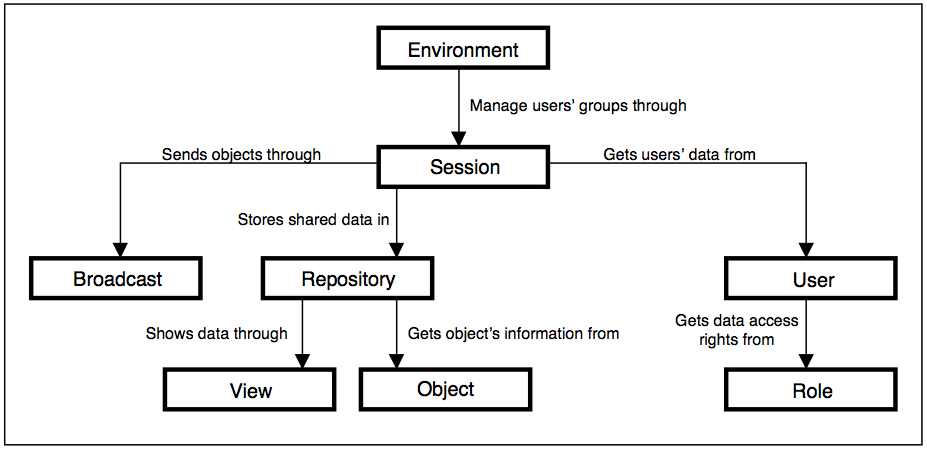
\includegraphics[width=1.0\textwidth]{images/chap5_pattern_system.png}
\caption{Pattern system of a collaborative system}
\label{fig:pattern_system}
\end{figure}

The environment object keeps track of all sessions in a collaborative application. A session can broadcast objects and is persisted through a user with a specific role. Furthermore, we have a Repository that is accessed through the session object and shown through a View.

\section{Collaboration Stack}

As we have seen in previous section, we have mapped the collaborative modeling framework onto the collaborative pattern system through several design patterns. These collaborative patterns can also regarded as a kind of documentation for a proven solution \cite{CollOntology}. In this section we will present an approach for creating an ontology of collaboration patterns and patterns languages. This ontology corresponds to a "collaboration stack" that identifies the various levels of abstraction. On one side we have some abstract collaboration patterns and on the other side we have the technologies that allow these patterns to be implemented.

\subsection{Ontology of collaboration patterns}

The collaboration stack is depicted in figure ~\ref{fig:coll_stack}. This stack was inspired by a typical IT protocol stack. Here we see the relation of collaboration patterns to collaborative services and their technologies. 

\begin{figure}[h!]
\centering
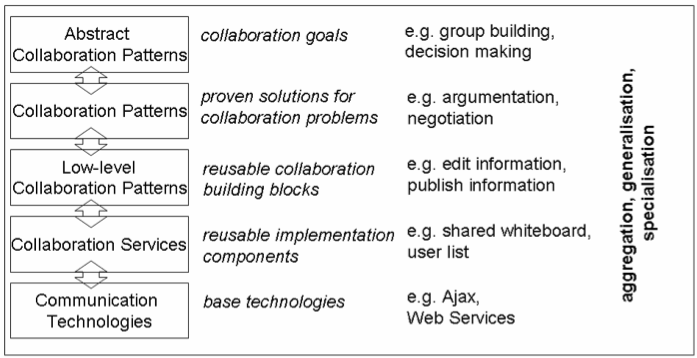
\includegraphics[width=0.9\textwidth]{images/chap5_coll_stack.png}
\caption{Collaboration Stack}
\label{fig:coll_stack}
\end{figure}

These collaboration patterns make use of their underlying services. For instance our environment pattern from the previous section makes use of the user list to handle sessions. In turn, these collaboration services make use of basic technologies. Now that we have a clear idea of our pattern system and the corresponding collaboration stack, we can describe the design of our collaborative framework. All components and their design will be described in the next chapter.
